\documentclass[12pt]{article}
\usepackage[margin=1in]{geometry}
\usepackage{amsfonts,amsmath,amssymb}
\usepackage[none]{hyphenat}
\usepackage{fancyhdr}
\usepackage{graphicx} 
\usepackage{float}
\usepackage{blindtext}
\usepackage{titlesec}
\usepackage[utf8]{inputenc}



\begin{document}
\begin{titlepage}
\begin{center}
\vspace{1cm}
\Large{\textbf{INDIAN INSTITUTE OF INFORMATION TECHNOLOGY KALYANI}}\\
\huge{\textbf{COMPUTER ORGANISATION AND ARCHITECTURE}}\\

\vfill
\line(1,0){400}\\[1mm]
\huge{\textbf{CARRY SAVE ADDER}}\\[3mm]
\Large{\textbf{Technical Report}}\\[1mm]
\line(1,0){400}\\
\vfill
RATNA PRIYA\\
39/CSE/17065/263\\
ratnpriya1998@gmail.com\\
\today\\
\end{center}
\end{titlepage}

\begin{abstract}
\textbf{This paper presents a technology-independent design and simulation of a modified architecture of 
the Carry-Save Adder. This architecture is shown to produce the result of the addition fast and by 
requiring a  minimum  number  of  logic gates.  Binary addition  is  carried out  by  a  series  of  XOR, 
AND  and  Shift-left  operations.  These  operations  are  terminated  with  a  completion  signal 
indicating  that  the  result  of  the  addition  is  obtained.  Because  the  number  of  shift  operations 
carried out varies from 0  to  n  for n-bit addends, a  behavioral model  was developed in which all 
the  possible  addends  having  2-  to  15-bits  were  applied. A  mathematical model  was deducted 
from  the  data  and  used  to  predict  the  average  number  of  shift  required  for  standard  binary 
numbers such as 32, 64 or 128-bits. 4-bit prototypes of this adder were designed and simulated 
in both synchronous and asynchronous modes of operation.}\cite{abstract} 
\end{abstract}

\section{INTRODUCTION}
Adders  are  commonly  found  in  the  critical path  of  many  building  blocks  of  microprocessors  and  digital  signal  processing  chips.  Adders  are  essential  not  only  for  addition,  but  also  for  subtraction,  multiplication,  and  division.  Addition  is  one  of  the  fundamental  arithmetic  operations.  A  fast  and  accurate  operation  of  a  digital  system  is  greatly  influenced  by  the  performance  of  the  resident  adders.  The  most  important  for  measuring the quality of adder designs in the past were propagation delay, and area.  In  array  processing  and  in  multiplication  and  division,  multioperand  addition  is  often  encountered.  More  powerful  adders  are  required  which  can  add  many  numbers  instead  of  two  together.  The  design  of  a  high-speed  multioperand  adder  called  Carry-Save  Adder  (CSA).  A  ripple  carry  adder  turns  into  a  carry-save-adder  if  the  carry  is  saved (stored) rather than propagate. The name ‘carry save’ arises from the fact that we save  the  carry-out  word  instead  of  using  it  immediately  to  calculate  a  final  sum.  The  principal  idea  is  that  the  carry  has  a  higher  power  of  2  and  thus  is  routed  to  the  next  column. Carry save adder is ideal to add several operands together. Thus, it can prevent time-consuming carry propagation and speed up computation. Effort the past shows that 16-bit  CSA  is  the  fastest  adder  within  another  adders  [Chetana  Nagendra,  Robert  Michael Owenz, and Mary Jane Irwin, 1996]. 
Carry-save-adder (CSA) is the most often used type of operation in implementing a fast computation of arithmetics of register-transfer-level design in industry. This paper establishes a relationship between the properties of arithmetic computations and several optimizing transformations using CSAs to derive consistently better qualities of results than those of manual implementations. In particular, we introduce two important concepts, operation duplication and operation split, which are the main driving techniques of our algorithm for achieving an extensive utilization of CSAs. Experimental results from a set of typical arithmetic computations found in industry designs indicate that automating CSA optimization with our algorithm produces designs with up to 53\% faster timing and up to 42\% smaller area.\cite{Intro}
\section{CARRY SAVE ADDER}
Carry  save  adder  is  used  to compute  sum  of  three  or  more  n-bit  binary  numbers. \\ Carry save 
adder is  same  as  a  full adder.\\ Figure shows the 4-bit and 3-bit carry save adders \\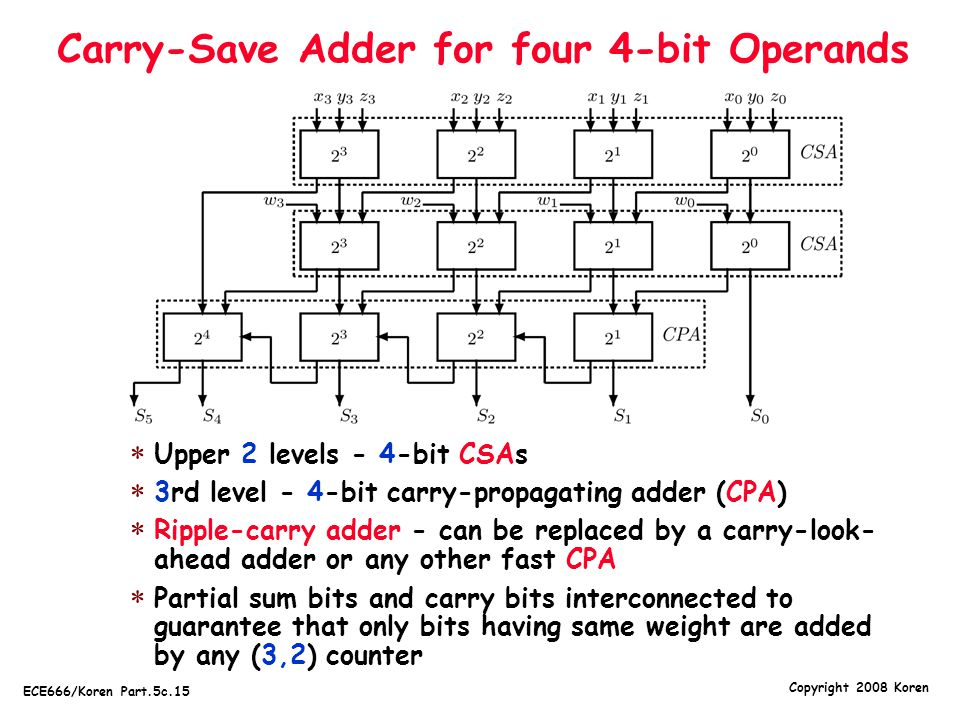
\includegraphics[scale=0.6]{csa-adder.jpg}\\
\\Carry save unit consists of 32 full adders, each of which computes 
single sum and carry  bit  based only  on  the corresponding bits of  the  two input  numbers.\\ \\ Let  X 
and Y  are two 32-bit  numbers and produces partial sum and carry  as S and C as  shown in the 
following example:\\ 
Si = Xi xor Yi\\ 
Ci = Xi and Yi \\ \\
The final addition is then computed as: \\
1. Shifting the carry sequence C left by one place.\\ 
2. Placing a 0 to the front (MSB) of the partial sum sequence S.\\ 
3. Finally, a ripple carry adder is used to add these two together and computing the resulting sum.\cite{csa} \\
\section{ADDITION IN CARRY SAVE ADDER}
The use of carry-save adders to efficiently compute a multioperand addition.
There are many circumstances in which we need to add a set of numbers together. For example, consider computing the inner product of two vectors of length n, A=[a1,a2,…,an]
and B=[b1,b2,…,bn.

 In this case, we need to compute $$A.B={A_{1}}{B_{1}}+{A_{2}}{B_{2}}+{A_{3}}{B_{3}}+.....+{A_{n}}{B_{n}}$$

As you can see, the inner product of two vectors of length n requires adding a set of n numbers together.
\subsection{MULTIOPERAND ADDITION USING A TWO OPERAND ADDER}
We can use a single two-operand adder sequentially to perform a multioperand addition.Assume that we need to add m numbers together, i.e., $$x_{0}+x_{2}+x_{3}+...+x_{n}$$Also, assume that the sum of these numbers, acc, can be represented by n bits. For this addition, we can use the block diagram\\
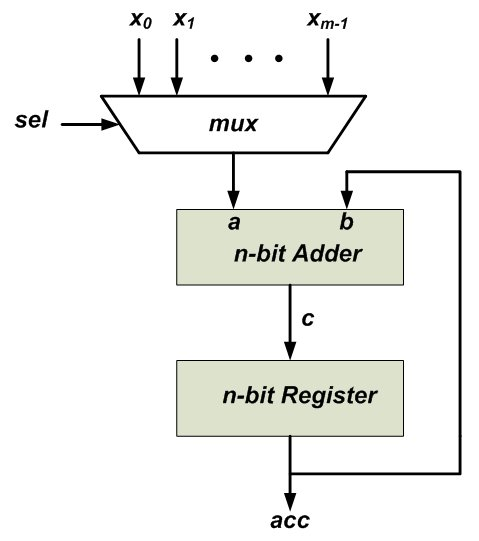
\includegraphics[scale=0.5]{mulop.jpg}\\

At the beginning of the calculations, the n-bit register is reset to zero. Then, the first operand, x0
, is selected by the multiplexer and applied to the n-bit adder. The other input of the adder, b, comes from the n-bit register. Hence, at this stage, the output of the n-bit adder will be c=x0+0=x0
. With the upcoming clock tick, this will be stored in the n-bit register, i.e. acc = x0

Next, the second operand, x1
, will be chosen by the multiplexer. This will be added to the current value of the n-bit register which gives c=x1+acc=x1+x0
. With the next clock edge, the value of the n-bit register will be acc=x1+x0
. This procedure will be repeated for the remaining operands. With each clock tick, a new operand will be added and the result will be stored in the n-bit register. Note that we’ll need a control unit to generate an appropriate signal for the select input of the multiplexer.\cite{Addition}
\section{APPLICATIONS OF CSA}
Instead of waiting for the carry propagation of the first addition, the idea here is to overlap the carry propagation of the first addition with the computation in the second addition,  and  so  forth,  since  repetitive  additions  will  be  performed  by  a  multioperandadder.  After  the  last  addition,  the  carry  propagation  delay  is  then  unavoidable  and  it  should be included in the total delay time.  When three or more operands are to be added simultaneously, using two operand adders,  the  time  consuming  carry-propagation  must  be  repeated  several  times.  If  the  number of operands is k, then carry has to propagate (k-1) times. Several techniques for multiple  operand  addition  that  attempt  to  lower  the  carry  propagation  have  been  proposed and implemented. 
\section*{ACKNOWLEDGMENT}
\textit{This project is a result of dedicated efforts. I would like to express my gratitude to Prof. Debashish Bera for able guidance and constructive suggestions.And I am grateful to everyone supporting out this project.}

\begin{thebibliography}{}
\bibitem{abstract}
IEEE Xplore, Digital Library, Circuit optimization using carry-save-adder cells\\https://ieeexplore.ieee.org/document/728918

\bibitem{Intro} A Hashim:(in 2007)\\http://dspace.unimap.edu.my/dspace/bitstream/123456789/1933/3/Introduction.pdf

\bibitem{csa} Chakib Alauli, Université Euro-Méditerranéenne de Fès, INSA EUROMED - Electrical Engineering, Articles and Published Reports

\bibitem{Addition} Steve Arar, contributing writer, All About Circuits\\
https://www.allaboutcircuits.com/technical-articles/use-carry-save-adders-efficiently\\-implement-multioperand-addition/


\end{thebibliography}

\end{document}

